\chapter{Trafic membranaire et adressage des protéines}\label{ch:b3:membrane-traffic}

Une cellule du pancréas fabrique quelque dix millions de molécules
d'enzyme digestive par minute, les emballe en granules et les libère
dans un canal sur un signal venu de l'intestin --- sans jamais laisser
une molécule de trypsine en liberté dans son propre cytoplasme. Une
cellule du foie retire le cholestérol du sang en avalant tout entières
les particules qui le transportent, à raison de quelques milliers par
minute, et renvoie chaque récepteur à la surface pour la suivante. Une
protéine fraîchement produite et destinée à la mitochondrie, au noyau,
au \omterm{def:b3:membrane-traffic:endocytosis}{lysosome}, à la membrane ou au monde extérieur atteint son adresse
parmi une douzaine de compartiments avec un taux d'erreur qui ferait
honte à un service postal. Ce chapitre traite de cet adressage~: les
signaux inscrits dans les protéines, les machines qui les lisent, les
vésicules qui portent membrane et cargaison d'un compartiment à
l'autre, les manteaux qui façonnent les vésicules et les protéines qui
les font fusionner avec la bonne cible, et le trafic à double sens ---
la sécrétion vers l'extérieur, l'endocytose vers l'intérieur --- qu'une
cellule eucaryote entretient à chaque seconde de sa vie.

\section{Signaux et adresses}

\begin{definition}[Les signaux d'adressage]\label{def:b3:membrane-traffic:signals}
\index{signal d'adressage}\index{peptide signal}\index{signal de localisation nucléaire}\index{préséquence}
Un \emph{signal d'adressage} est un segment d'une protéine, ou une
modification de celle-ci, que lit un récepteur qui livre la protéine à
un compartiment. Le \emph{peptide signal}, suite de
\numrange{15}{30} résidus à l'extrémité aminée dotée d'un cœur
hydrophobe, envoie une protéine dans le réticulum endoplasmique pendant
qu'elle se fait~; de là, la voie par défaut passe par le Golgi et mène
à la membrane plasmique ou à l'extérieur, et d'autres signaux détournent
vers le \omterm{def:b3:membrane-traffic:endocytosis}{lysosome} (un sucre phosphorylé) ou en arrière vers le réticulum
(la séquence carboxy-terminale KDEL). Un \emph{signal de localisation
nucléaire}, court îlot basique tel que PKKKRKV, est reconnu par des
importines qui font passer la protéine repliée par le pore nucléaire~;
une \emph{préséquence} mitochondriale, hélice amphipathique de
\numrange{20}{50} résidus, est reconnue par des récepteurs de la
membrane externe et enfilée, dépliée, à travers les translocases des
deux membranes~; les enzymes peroxysomales se terminent par SKL. Les
protéines qui n'ont aucun de ces signaux restent dans le cytosol.
Chaque signal a été trouvé de la même manière~: le supprimer laisse la
protéine dans le cytosol, le greffer sur une protéine cytosolique
envoie celle-ci dans le compartiment.
\end{definition}

\begin{proof}[Faits expérimentaux]
Blobel et Dobberstein (1975) ont traduit l'ARN messager d'une chaîne
légère d'anticorps dans un système acellulaire. Sans membranes, le
produit était plus long d'une vingtaine de résidus que la protéine
sécrétée~; avec des fragments de réticulum endoplasmique ajoutés
\emph{pendant} la traduction, le produit avait la taille de la protéine
sécrétée et était protégé d'une protéase ajoutée --- il était à
l'intérieur des vésicules --- alors que des membranes ajoutées après la
traduction ne changeaient rien. Le segment amino-terminal
supplémentaire, le \omterm{def:b3:membrane-traffic:signals}{peptide signal}, est nécessaire pour entrer dans le
réticulum, y est retiré, et ne fonctionne que pendant que la chaîne se
fait~: c'est l'\emph{hypothèse du signal}, confirmée dans le moindre
détail lorsque le récepteur (la particule de reconnaissance du signal,
Walter et Blobel 1981) et le canal (Sec61) ont été purifiés.
\end{proof}

\begin{omfigure}
\begin{tikzpicture}[every node/.style={font=\scriptsize}, >=stealth]
  % ER membrane
  \fill[omDef!15] (0,0) rectangle (12,-1.6);
  \draw[very thick, omDef] (0,0) -- (12,0); \draw[very thick, omDef] (0,-0.35) -- (12,-0.35);
  \node[right, omDef!70!black] at (0.1,-1.3) {lumière du RE};
  \node[right] at (0.1,2.9) {cytosol};
  % stage 1: ribosome with emerging signal peptide + SRP
  \draw[thick, fill=gray!25] (1.4,1.6) circle (0.5); \draw[thick, fill=gray!25] (1.4,0.95) ellipse (0.62 and 0.3);
  \draw[very thick, omThm] (1.4,0.65) -- (1.4,0.2) -- (1.9,0.1);
  \draw[thick, fill=omProp!40] (2.1,0.35) ellipse (0.35 and 0.2); \node[above right] at (2.2,0.5) {SRP};
  \node[below, align=center] at (1.7,-1.7) {1. le peptide signal émerge~;\\la SRP se fixe, la traduction pause};
  % stage 2: docking at SRP receptor and translocon
  \draw[->, thick] (3.2,1.2) -- (4.2,1.2);
  \draw[thick, fill=gray!25] (5.6,1.75) circle (0.5); \draw[thick, fill=gray!25] (5.6,1.1) ellipse (0.62 and 0.3);
  \draw[thick, fill=omMeth!40] (5.2,0.0) rectangle (5.45,-0.35); \draw[thick, fill=omMeth!40] (5.75,0.0) rectangle (6.0,-0.35);
  \node[below, align=center] at (5.9,-1.7) {2. le récepteur de la SRP l'amarre\\sur Sec61~; la SRP s'en va};
  \draw[very thick, omThm] (5.6,0.8) -- (5.6,-0.2);
  \draw[thick, fill=omProp!40] (4.7,0.15) ellipse (0.3 and 0.18); \node[above] at (4.7,0.33) {récepteur de la SRP};
  % stage 3: translocation, cleavage, glycosylation
  \draw[->, thick] (7.2,1.2) -- (8.2,1.2);
  \draw[thick, fill=gray!25] (9.6,1.75) circle (0.5); \draw[thick, fill=gray!25] (9.6,1.1) ellipse (0.62 and 0.3);
  \draw[thick, fill=omMeth!40] (9.2,0.0) rectangle (9.45,-0.35); \draw[thick, fill=omMeth!40] (9.75,0.0) rectangle (10.0,-0.35);
  \draw[very thick, omThm] (9.6,0.8) -- (9.6,-0.5) .. controls (9.6,-1.0) and (10.3,-1.1) .. (10.6,-0.7);
  \draw[omThm, thick] (10.9,-0.9) -- (11.2,-0.9); \node[right, font=\tiny] at (11.0,-1.15) {signal coupé};
  \fill[omExo] (10.3,-1.0) circle (0.07); \fill[omExo] (10.45,-1.12) circle (0.07); \node[below, font=\tiny] at (10.2,-1.15) {sucres};
  \node[below, align=center] at (10.0,-1.7) {3. la chaîne traverse en se faisant~;\\signal coupé, sucres ajoutés};
\end{tikzpicture}

{\small L'hypothèse du signal. Un \omterm{def:b3:membrane-traffic:signals}{peptide signal} en tête de la chaîne
naissante est reconnu par la particule de reconnaissance du signal, qui
met la traduction en pause et amarre le ribosome sur le canal Sec61~;
la chaîne traverse alors la membrane à mesure qu'elle est synthétisée,
le signal est coupé dans la lumière, et des sucres sont ajoutés.}
\end{omfigure}

\begin{proposition}[Protéines membranaires et topologie]\label{prop:b3:membrane-traffic:topology}
\index{séquence d'arrêt de transfert}\index{topologie membranaire}
Un tronçon hydrophobe d'une vingtaine de résidus au milieu d'une chaîne
en cours de translocation agit comme une \emph{\omterm{prop:b3:membrane-traffic:topology}{séquence d'arrêt de
transfert}}~: le canal s'ouvre latéralement et la libère dans la
bicouche sous forme d'hélice transmembranaire, la part déjà transloquée
restant dans la lumière et le reste se faisant dans le cytosol. Un
second tronçon de ce genre relance la translocation, et une protéine
munie de $n$ signaux alternés finit avec $n$ hélices
transmembranaires. L'orientation fixée dans le réticulum n'est jamais
changée~: ce qui fait face à la lumière du réticulum fait face à la
lumière du Golgi et de toute vésicule ensuite, et à l'\emph{extérieur}
de la cellule après fusion avec la membrane plasmique. Les sucres,
ajoutés seulement dans la lumière, sont donc toujours sur la face
extracellulaire d'une protéine de surface, et la topologie d'un
récepteur se lit à l'emplacement de ses sites de glycosylation.
\end{proposition}

\begin{method}[Marquage et chasse]\label{met:b3:membrane-traffic:pulse-chase}
\index{marquage--chasse}\index{autoradiographie}
Pour suivre à travers la cellule une population de molécules
fraîchement produites~: (1) exposer brièvement les cellules (le
\emph{marquage}, quelques minutes) à un précurseur radioactif ou
autrement marqué --- de la leucine tritiée pour les protéines~;
(2) le remplacer par un excès de précurseur non marqué (la
\emph{chasse}), de sorte qu'aucun marqueur neuf ne soit incorporé~;
(3) fixer des échantillons de cellules à intervalles réguliers et
localiser le marqueur par autoradiographie sur des micrographies
électroniques, ou en isolant les compartiments et en comptant~;
(4) porter la fraction de marqueur de chaque compartiment en fonction
du temps. L'ordre dans lequel les compartiments se remplissent et se
vident est la route~; la chronologie donne le temps de séjour dans
chacun. Le laboratoire de Palade (années 1960) l'a appliqué à la
cellule acineuse du pancréas et a trouvé le marqueur dans le réticulum
rugueux à \qty{3}{min}, dans le Golgi à \qty{20}{min}, dans les
vacuoles de condensation et les granules à \qty{40}{min}, et dans le
canal après une heure et sur un signal~: la voie de sécrétion, déployée
dans le temps.
\end{method}

\begin{theorem}[Compartiments successifs et courbes de marquage--chasse]\label{thm:b3:membrane-traffic:pulse-chase}
\index{modèle à compartiments}
Soit une impulsion de protéine marquée qui quitte le compartiment $A$
pour $B$ à la vitesse du premier ordre $k_{1}$ et quitte $B$ pour $C$ à
la vitesse $k_{2}$, $C$ la retenant. Tout le marqueur étant dans $A$ en
$t = 0$,
\[
A(t) = e^{-k_{1}t},\qquad
B(t) = \frac{k_{1}}{k_{2} - k_{1}}\bigl(e^{-k_{1}t} - e^{-k_{2}t}\bigr),
\qquad
C(t) = 1 - A - B,
\]
et le marqueur présent dans $B$ passe par un maximum en
$t^{*} = \ln(k_{2}/k_{1})/(k_{2} - k_{1})$. Le temps de séjour moyen
dans $A$ vaut $1/k_{1}$ et dans $B$ vaut $1/k_{2}$, quel que soit
l'ordre des deux vitesses.
\end{theorem}
\begin{proof}
$\mathrm{d}A/\mathrm{d}t = -k_{1}A$ donne l'exponentielle. Pour $B$,
$\mathrm{d}B/\mathrm{d}t = k_{1}A - k_{2}B = k_{1}e^{-k_{1}t} - k_{2}B$~;
essayons $B = \beta(e^{-k_{1}t} - e^{-k_{2}t})$~: la dérivée vaut
$\beta(-k_{1}e^{-k_{1}t} + k_{2}e^{-k_{2}t})$ et $-k_{2}B = \beta(-k_{2}
e^{-k_{1}t} + k_{2}e^{-k_{2}t})$, de sorte que l'équation exige $\beta(k_{2}
- k_{1})e^{-k_{1}t} = k_{1}e^{-k_{1}t}$, $\beta = k_{1}/(k_{2} -
k_{1})$, et $B(0) = 0$ comme il se doit. En posant
$\mathrm{d}B/\mathrm{d}t =
0$~: $k_{1}e^{-k_{1}t} = k_{2}e^{-k_{2}t}$, d'où $t^{*}$. Le temps moyen
qu'une molécule passe dans un compartiment qu'elle quitte à la vitesse
$k$ vaut $\int_{0}^{
\infty} t\,k e^{-kt}\,\mathrm{d}t = 1/k$.
\end{proof}

\begin{example}[La cellule de Palade en chiffres]\label{ex:b3:membrane-traffic:palade}
Prenons $k_{1} = \qty{0.1}{min^{-1}}$ (dix minutes dans le réticulum) et
$k_{2} = \qty{0.05}{min^{-1}}$ (vingt dans le Golgi). Le Golgi passe par
son maximum en $t^{*} = \ln 2/0.05 = \qty{13.9}{min}$, retenant alors
$B = 2(e^{-1.39} -
e^{-0.69}) = 2(0.25 - 0.50)\cdot(-1) = 0.50$~: la moitié du marqueur. À
\qty{40}{min}, $A = 0.018$, $B = 2(0.018 - 0.135) \to 0.23$, $C = 0.75$~:
les trois quarts de la protéine ont atteint les granules. Les courbes
observées par le laboratoire de Palade ont cette allure, et c'est en
les ajustant que les temps de séjour ont été mesurés pour la première
fois.
\end{example}

\begin{omfigure}
\begin{tikzpicture}
\begin{axis}[
  width=0.7\linewidth, height=5.6cm,
  axis x line=bottom, axis y line=left,
  xmin=0, xmax=80, ymin=0, ymax=1.05,
  xlabel={minutes après le marquage}, ylabel={fraction du marqueur},
  xlabel style={font=\small, at={(axis description cs:0.5,-0.12)}, anchor=north},
  ylabel style={font=\small},
  tick label style={font=\small}, xtick={0,20,40,60,80}, ytick={0,0.5,1},
  clip=false,
]
\addplot[very thick, omDef, domain=0:80, samples=80] {exp(-0.1*x)};
\addplot[very thick, omProp, domain=0:80, samples=80] {2*(exp(-0.05*x)-exp(-0.1*x))};
\addplot[very thick, omMeth!70!black, domain=0:80, samples=80] {1-exp(-0.1*x)-2*(exp(-0.05*x)-exp(-0.1*x))};
\node[font=\scriptsize, omDef, anchor=south west] at (axis cs:4,0.62) {réticulum, $A$};
\node[font=\scriptsize, omProp, anchor=south] at (axis cs:14,0.53) {Golgi, $B$};
\node[font=\scriptsize, omMeth!70!black, anchor=north west] at (axis cs:45,0.72) {granules, $C$};
\end{axis}
\end{tikzpicture}

{\small Courbes de marquage--chasse données par le modèle à deux
vitesses avec $k_{1} =
\qty{0.1}{min^{-1}}$ et $k_{2} = \qty{0.05}{min^{-1}}$~: le marqueur
quitte le réticulum exponentiellement, traverse le Golgi avec un
maximum à \qty{14}{min}, et s'accumule dans les granules.}
\end{omfigure}

\section{Le réticulum endoplasmique~: repliement, sucres et qualité}

\begin{definition}[N-glycosylation et contrôle qualité]\label{def:b3:membrane-traffic:glycosylation}
\index{N-glycosylation}\index{cycle de la calnexine}\index{dégradation associée au réticulum}\index{réponse aux protéines mal repliées}
À mesure que la chaîne entre dans la lumière, un oligosaccharide
préassemblé de quatorze sucres (deux N-acétylglucosamines, neuf
mannoses, trois glucoses) est transféré depuis un porteur lipidique sur
des asparagines de la séquence Asn-X-Ser/Thr --- la
\emph{N-glycosylation}. Les trois glucoses sont ensuite retirés un à
un, et ce retrait est une horloge du \omterm{def:b3:structural-biology:levels}{repliement}~: une protéine qui
porte encore un glucose est retenue par le \omterm{def:b3:structural-biology:chaperones}{chaperon} calnexine~; une
protéine dont le dernier glucose a été retiré mais qui n'est pas encore
repliée est reglucosylée par une enzyme qui reconnaît les zones
hydrophobes exposées, et retourne à la calnexine --- c'est le
\emph{cycle de la calnexine}. Les protéines qui échouent à répétition
sont ramenées dans le cytosol, ubiquitinylées et détruites par le
protéasome~: c'est la \emph{dégradation associée au réticulum} (ERAD).
Quand les protéines mal repliées s'accumulent plus vite qu'on ne peut
les replier ou les détruire, des capteurs de la membrane du réticulum
déclenchent la \emph{réponse aux protéines mal repliées}~: la
traduction est ralentie, les gènes de \omterm{def:b3:structural-biology:chaperones}{chaperons} induits, le réticulum
étendu et, si la contrainte persiste, la cellule tuée. La mutation la
plus fréquente de la mucoviscidose ($\Delta$F508 dans CFTR) donne un
canal qui fonctionnerait mais se replie trop lentement, est attrapé par
l'ERAD et n'atteint jamais la surface~; des médicaments qui l'aident à
se replier sont aujourd'hui un traitement.
\end{definition}

\begin{omfigure}
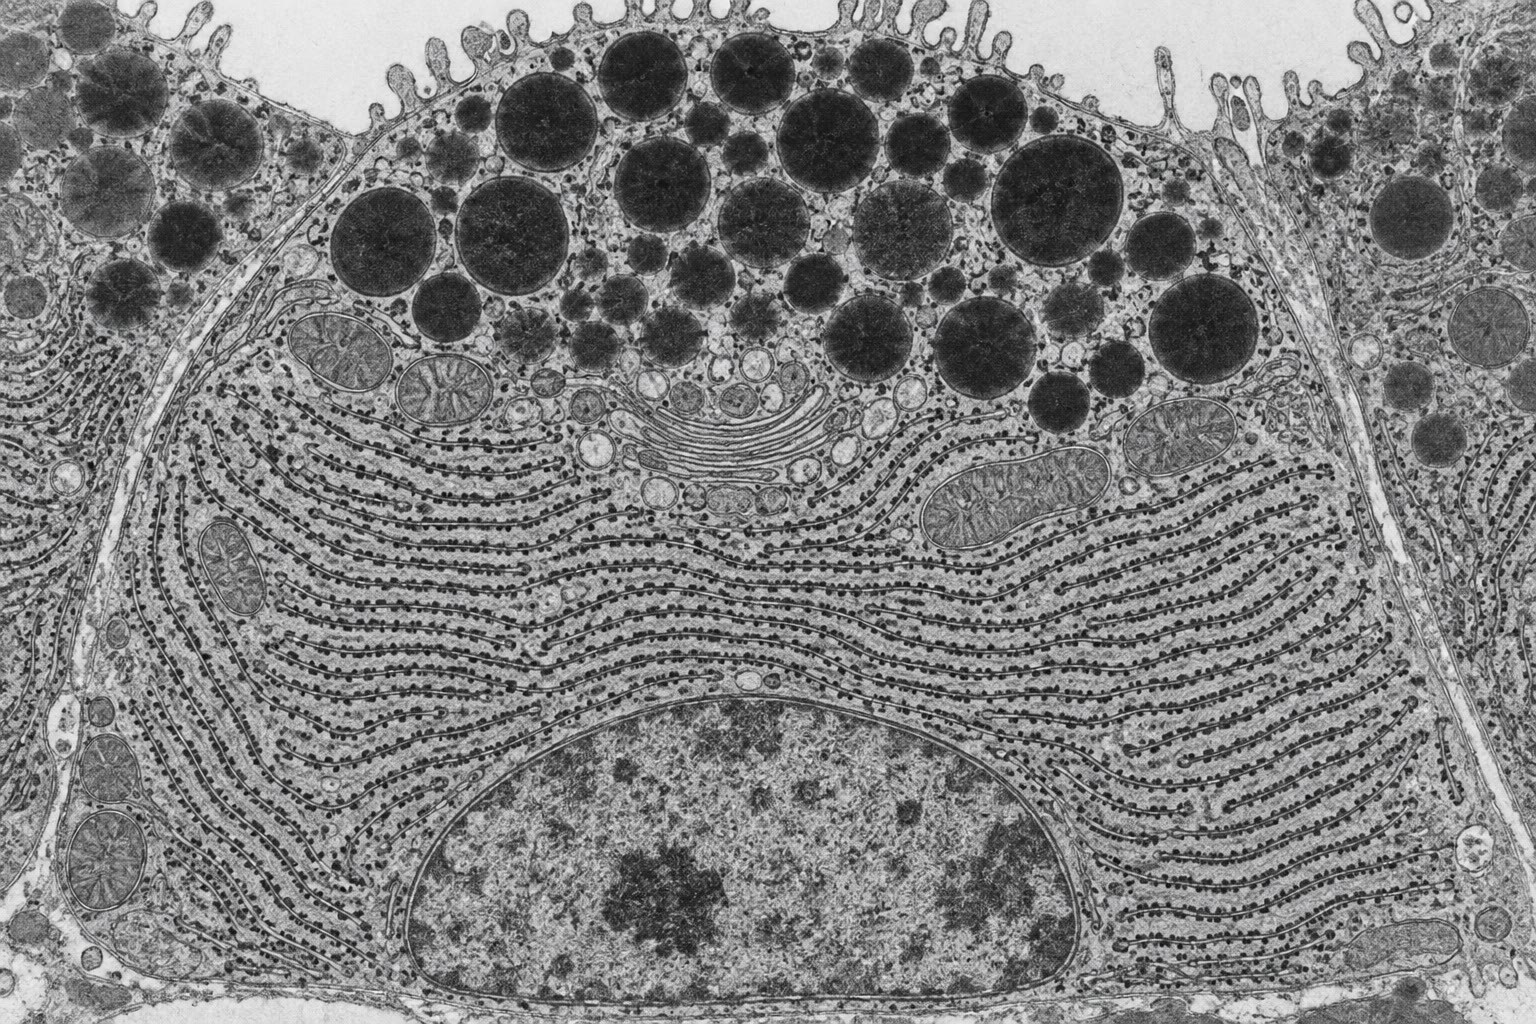
\includegraphics[width=0.56\linewidth]{images/book5/ai/b5-08-pancreas-acinar.jpg}

{\small Une cellule acineuse du pancréas au microscope électronique~:
des empilements de réticulum endoplasmique rugueux hérissé de ribosomes
remplissent la base, le Golgi se tient au-dessus du noyau, et des
granules de sécrétion denses, pleins d'enzymes digestives, sont tassés
sous la surface apicale, attendant un signal.}
\end{omfigure}

\section{Les vésicules~: bourgeonnement, adressage, fusion}

\begin{definition}[Manteaux et bourgeonnement des vésicules]\label{def:b3:membrane-traffic:coats}
\index{vésicule à manteau}\index{COPII}\index{COPI}\index{clathrine}\index{petite GTPase}
Une vésicule de transport est façonnée par un \emph{manteau} de
protéines assemblé sur la face cytosolique d'une membrane, qui courbe
celle-ci en un bourgeon de \qtyrange{60}{100}{nm}, rassemble la
cargaison grâce à des récepteurs qui traversent la membrane, et se
défait une fois la vésicule détachée. Trois manteaux desservent les
routes principales~: \emph{COPII} pour les vésicules qui quittent le
réticulum vers le Golgi, \emph{COPI} pour le trafic de retour du Golgi
vers le réticulum et entre citernes golgiennes, et la
\emph{clathrine} --- protéine à trois pieds qui polymérise en une cage
d'hexagones et de pentagones --- pour les vésicules qui quittent le
Golgi trans vers les \omterm{def:b3:membrane-traffic:endocytosis}{endosomes} et pour l'endocytose à la membrane
plasmique, où des protéines adaptatrices relient la cage aux récepteurs
à internaliser. Chaque manteau est recruté par une \emph{petite GTPase}
(Sar1 pour COPII, Arf1 pour COPI et la clathrine) qui s'insère dans la
membrane sous sa forme GTP et, en hydrolysant le GTP après le
bourgeonnement, laisse tomber le manteau. Des signaux de récupération
maintiennent les compartiments distincts~: les protéines du réticulum
échappées et porteuses de KDEL sont reconnues dans le Golgi par un
récepteur et ramenées dans des vésicules COPI.
\end{definition}

\begin{omfigure}
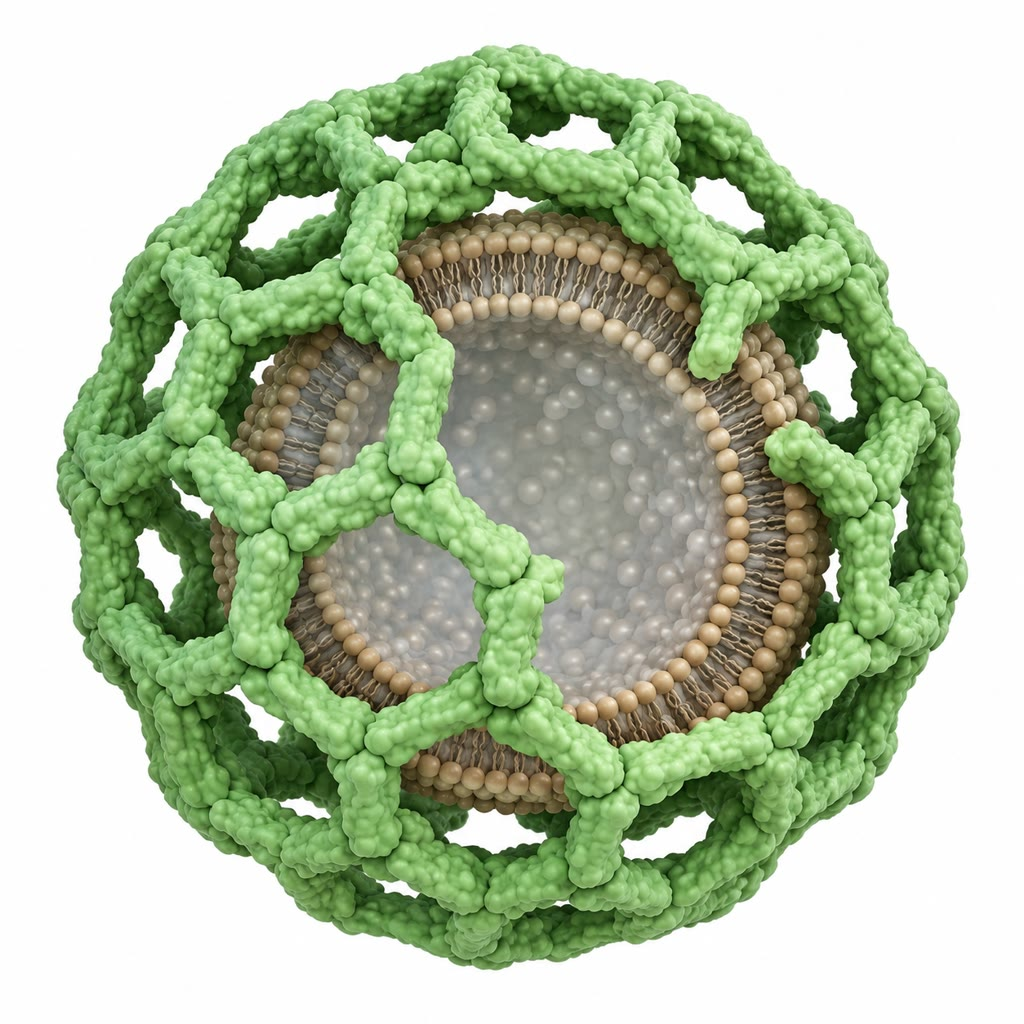
\includegraphics[width=0.36\linewidth]{images/book5/ai/b5-08-clathrin-cage.jpg}\hspace{0.04\linewidth}
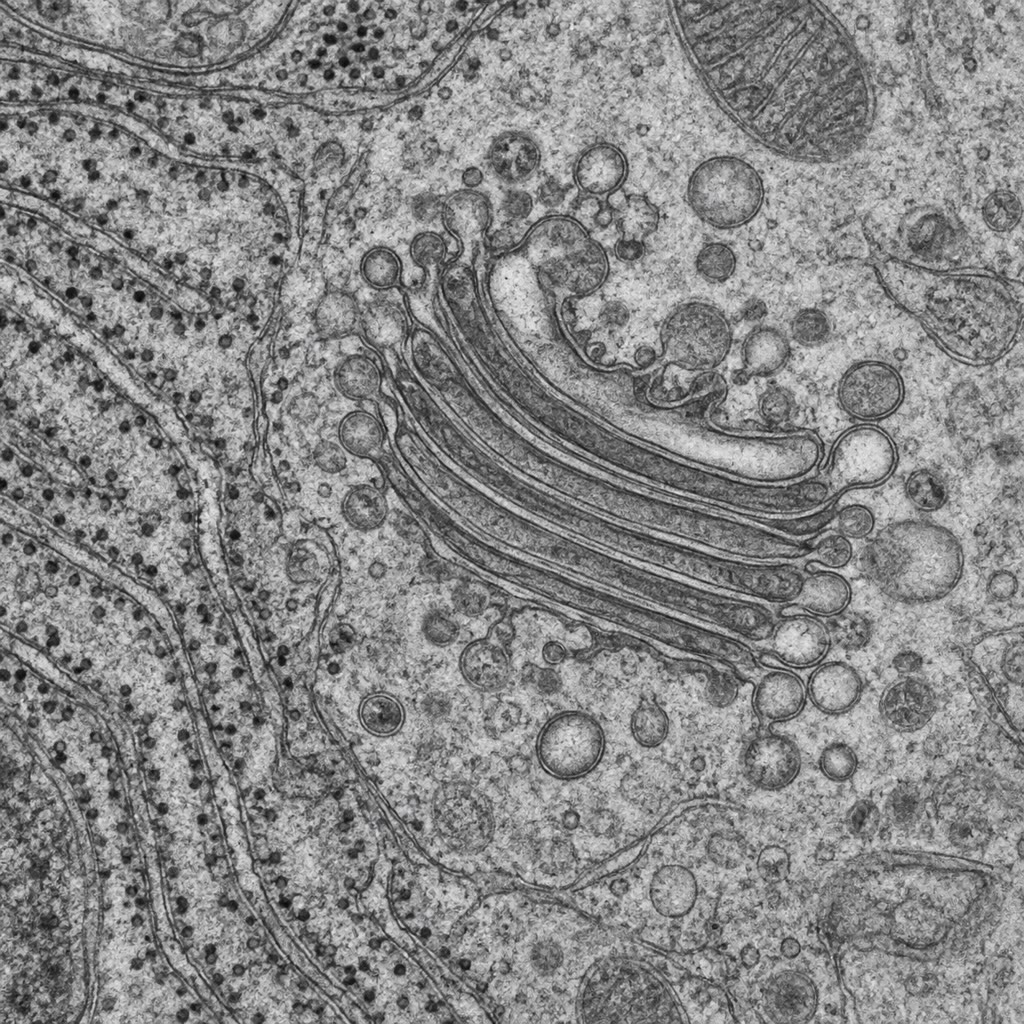
\includegraphics[width=0.36\linewidth]{images/book5/ai/b5-08-golgi-tem.jpg}

{\small À gauche~: une cage de \omterm{def:b3:membrane-traffic:coats}{clathrine}, le réseau polyédrique d'unités
à trois pieds qui façonne une vésicule d'endocytose (écorchée pour
montrer la membrane à l'intérieur). À droite~: un dictyosome au
microscope électronique, une pile de citernes aplaties d'où bourgeonnent
des vésicules sur les bords.}
\end{omfigure}

\begin{definition}[Adressage et fusion]\label{def:b3:membrane-traffic:fusion}
\index{GTPase Rab}\index{SNARE}\index{fusion membranaire}\index{synaptotagmine}
Une vésicule trouve sa cible par deux couches de reconnaissance. Les
\emph{GTPases Rab} --- une soixantaine dans une cellule humaine,
chacune sur les membranes d'un compartiment --- recrutent de longues
protéines d'amarrage qui attrapent une vésicule entrante porteuse de la
Rab correspondante. Puis les \emph{SNARE} agissent~: une v-SNARE sur la
vésicule et des t-SNARE sur la cible, protéines hélicoïdales ancrées
dans leurs membranes, s'enroulent l'une autour de l'autre depuis leurs
extrémités distales vers les membranes, et l'énergie du faisceau à
quatre hélices qu'elles forment tire les deux bicouches l'une contre
l'autre jusqu'à la fusion. Chaque appariement de SNARE est spécifique,
seconde vérification de l'adresse. Après la fusion, le faisceau est
défait par l'ATPase NSF pour être réemployé. On peut faire attendre la
fusion jusqu'à un signal~: dans la terminaison nerveuse, les SNARE sont
tenues à demi fermées par la complexine jusqu'à ce que la
\emph{synaptotagmine}, en fixant le calcium qui entre à l'arrivée d'un
potentiel d'action, achève la fermeture éclair en moins d'une
milliseconde --- la libération du neurotransmetteur, traitée dans le
volume de deuxième année. Les neurotoxines du tétanos et du botulisme
sont des protéases qui clivent des SNARE.
\end{definition}

\begin{proof}[Faits expérimentaux]
Novick et Schekman (1980) ont isolé des mutants de levure thermosensibles
qui cessaient de sécréter à \qty{37}{\celsius} et accumulaient de la
protéine dans le compartiment que bloquait leur défaut --- réticulum,
Golgi ou vésicules entassées sous la surface~; les $23$ gènes
\emph{sec} ont défini les étapes et, une fois clonés, se sont révélés
coder les manteaux, les GTPases et les \omterm{def:b3:membrane-traffic:fusion}{SNARE}. Rothman a reconstitué le
transport entre citernes golgiennes dans un tube à essai, avec des
membranes purifiées, du cytosol et de l'ATP, et en a purifié NSF et les
\omterm{def:b3:membrane-traffic:fusion}{SNARE}~; les deux approches ont convergé vers les mêmes protéines, et les
machines de levure et de mammifère se sont révélées être les mêmes.
\end{proof}

\begin{omfigure}
\begin{tikzpicture}[every node/.style={font=\scriptsize}, >=stealth]
  % three stages left to right
  \foreach \x/\gap/\lab in {0/1.2/{1. amarrée par une Rab}, 4.4/0.55/{2. les SNARE se ferment}, 8.8/0.0/{3. fusion, cargaison libérée}} {
    % target membrane
    \draw[very thick, omDef] (\x,0) -- (\x+3.4,0); \draw[very thick, omDef] (\x,-0.3) -- (\x+3.4,-0.3);
    \node[below, align=center] at (\x+1.7,-0.45) {\lab};
  }
  % stage 1 vesicle
  \draw[very thick, omProp] (1.7,1.2+0.8) circle (0.8); \draw[very thick, omProp] (1.7,1.2+0.8) circle (0.6);
  \draw[omThm, thick] (1.4,1.25) -- (1.4,0.35); \draw[omThm, thick] (2.0,1.25) -- (2.0,0.35);
  \draw[omMeth!70!black, thick] (1.7,1.2) -- (1.7,0.6); \draw[omMeth!70!black, thick] (1.7,0.6) -- (1.7,0.0);
  \draw[thick, fill=omExo!40] (0.7,0.9) ellipse (0.25 and 0.2); \node[left] at (0.45,0.9) {Rab};
  \draw[thick, omExo!70!black] (0.95,0.9) .. controls (1.1,0.5) .. (1.2,0.05); \node[left, font=\tiny] at (0.9,0.4) {amarre};
  \node[right, font=\tiny] at (2.05,0.8) {SNAREs};
  % stage 2 vesicle closer, helices twisted
  \draw[very thick, omProp] (6.1,0.55+0.8) circle (0.8); \draw[very thick, omProp] (6.1,0.55+0.8) circle (0.6);
  \draw[omThm, very thick] (5.85,0.6) .. controls (6.2,0.5) and (5.9,0.3) .. (6.1,0.05);
  \draw[omMeth!70!black, very thick] (6.35,0.6) .. controls (6.0,0.5) and (6.3,0.3) .. (6.1,0.05);
  \node[right, font=\tiny, align=left] at (6.6,0.35) {le faisceau à quatre hélices\\tire les membranes\\l'une contre l'autre};
  % stage 3 fused omega shape
  \draw[very thick, omProp] (9.7,0) .. controls (9.7,1.5) and (11.3,1.5) .. (11.3,0);
  \draw[very thick, omProp] (9.9,-0.3) .. controls (9.9,1.1) and (11.1,1.1) .. (11.1,-0.3);
  \foreach \p in {(10.5,-0.9),(10.2,-1.1),(10.8,-1.15)} \fill[omExo] \p circle (0.06);
  \draw[->, omExo, thick] (10.5,0.5) -- (10.5,-0.6);
  \node[right, font=\tiny, align=left] at (11.4,0.8) {NSF défera\\ensuite les\\SNARE};
\end{tikzpicture}

{\small La fusion en trois temps. Une Rab sur la vésicule et une amarre
sur la cible rapprochent les deux membranes~; les \omterm{def:b3:membrane-traffic:fusion}{SNARE} de la vésicule
et de la cible (rouge et vert) se ferment en un faisceau à quatre
hélices qui tire les bicouches l'une contre l'autre~; elles fusionnent
et la cargaison entre dans le compartiment cible.}
\end{omfigure}

\begin{proposition}[Le Golgi]\label{prop:b3:membrane-traffic:golgi}
\index{appareil de Golgi}\index{maturation des citernes}\index{mannose-6-phosphate}
Le Golgi est une pile de quatre à huit citernes aplaties, face cis vers
le réticulum, face trans vers la membrane plasmique, chaque citerne
abritant un jeu d'enzymes différent qui rogne et reconstruit les sucres
des glycoprotéines de passage et ajoute des sucres O-liés, du sulfate
et du phosphate. La cargaison avance surtout par \emph{\omterm{prop:b3:membrane-traffic:golgi}{maturation des
citernes}}~: une nouvelle citerne se forme à la face cis à partir des
vésicules qui arrivent, progresse à travers la pile comme l'ont fait
celles qui la précèdent, et mûrit à mesure que des vésicules \omterm{def:b3:membrane-traffic:coats}{COPI}
rapportent les enzymes de chaque citerne à la plus jeune derrière
elle~; à la face trans elle se fragmente en vésicules destinées à leurs
adresses. C'est là que se décide l'adressage~: les hydrolases
lysosomales, marquées dans le Golgi cis d'un
\emph{mannose-6-phosphate}, sont reconnues par leur récepteur et
emballées dans des vésicules à \omterm{def:b3:membrane-traffic:coats}{clathrine} à destination de l'\omterm{def:b3:membrane-traffic:endocytosis}{endosome}~;
les protéines de sécrétion régulée s'agrègent au pH légèrement acide en
granules de condensation~; tout le reste part dans le flux constitutif
vers la surface. Dans la maladie des cellules à inclusions, l'enzyme
phosphorylante manque, les hydrolases sont sécrétées au lieu d'être
livrées, et les \omterm{def:b3:membrane-traffic:endocytosis}{lysosomes} se remplissent de matériel non digéré.
\end{proposition}

\begin{omfigure}
\begin{tikzpicture}[every node/.style={font=\scriptsize}, >=stealth]
  % plasma membrane top
  \draw[very thick, omDef] (0,4.2) -- (12,4.2); \node[above] at (6,4.25) {membrane plasmique \quad (extérieur au-dessus)};
  % ER
  \draw[thick, fill=omDef!12] (0.3,0.0) rectangle (4.0,0.9); \node at (2.15,0.45) {réticulum endoplasmique};
  % Golgi stack
  \foreach \y in {1.5,1.85,2.2,2.55} \draw[thick, fill=omProp!25] (4.8,\y) ellipse (1.4 and 0.13);
  \node[right] at (6.3,1.5) {cis}; \node[left] at (3.35,2.55) {trans};
  \node[right] at (6.3,2.05) {pile golgienne};
  % ER -> Golgi (COPII)
  \draw[->, thick, omMeth!70!black] (3.9,0.95) -- (4.5,1.4); \node[right, omMeth!70!black, font=\tiny] at (4.35,1.02) {COPII};
  % Golgi -> ER (COPI)
  \draw[->, thick, omThm] (3.6,1.42) -- (2.9,0.95); \node[left, omThm, font=\tiny] at (2.95,1.3) {COPI, récupération KDEL};
  % trans Golgi -> PM constitutive
  \draw[->, thick, omMeth!70!black] (5.6,2.7) -- (7.6,4.1); \node[left, font=\tiny, align=right] at (6.4,3.6) {sécrétion\\constitutive};
  % trans -> secretory granule -> PM regulated
  \draw[->, thick, omMeth!70!black] (4.6,2.7) -- (4.0,3.3); \draw[thick, fill=omExo!50] (3.8,3.5) circle (0.22); \draw[->, thick, omMeth!70!black] (3.8,3.75) -- (3.8,4.1);
  \node[left, font=\tiny, align=right] at (3.55,3.5) {granule de sécrétion~:\\régulée, sur un signal};
  % trans -> endosome/lysosome (clathrin, M6P)
  \draw[->, thick, omProp!80!black] (6.0,2.62) -- (8.25,2.62); \node[above, font=\tiny] at (7.1,2.67) {clathrine, récepteur M6P};
  \draw[thick, fill=omProp!20] (8.8,2.7) circle (0.5); \node at (8.8,2.7) {\tiny endosome};
  \draw[->, thick, omProp!80!black] (9.25,2.4) -- (10.2,1.95); \draw[thick, fill=omThm!25] (10.7,1.6) circle (0.5); \node at (10.7,1.6) {\tiny lysosome};
  % endocytosis from PM to endosome
  \draw[->, thick, omDef] (9.6,4.15) -- (9.1,3.2); \node[right, font=\tiny, align=left] at (9.5,3.7) {endocytose\\(puits à clathrine)};
  % recycling endosome -> PM
  \draw[->, thick, omDef] (8.5,3.2) -- (8.0,4.15); \node[left, font=\tiny] at (8.3,3.3) {recyclage};
  % lysosome inputs autophagy
  \draw[->, thick, gray] (11.9,0.6) -- (11.1,1.3); \node[below, font=\tiny, align=center] at (11.9,0.55) {autophagosome\\(cytoplasme, organites)};
\end{tikzpicture}

{\small La carte du trafic membranaire. Vers l'extérieur (vert)~: du
réticulum au Golgi dans des vésicules \omterm{def:b3:membrane-traffic:coats}{COPII}, du Golgi à la surface soit
de façon constitutive, soit par des granules qui attendent un signal.
Vers l'arrière (rouge)~: des vésicules \omterm{def:b3:membrane-traffic:coats}{COPI} ramènent les protéines
échappées du réticulum. Vers le bas (orange)~: les enzymes lysosomales
marquées au mannose-6-phosphate gagnent l'\omterm{def:b3:membrane-traffic:endocytosis}{endosome} et le \omterm{def:b3:membrane-traffic:endocytosis}{lysosome}. Vers
l'intérieur (bleu)~: l'endocytose depuis la surface, la plupart des
récepteurs étant recyclés.}
\end{omfigure}

\section{L'endocytose et le lysosome}

\begin{definition}[L'endocytose]\label{def:b3:membrane-traffic:endocytosis}
\index{endocytose par récepteurs interposés}\index{endosome}\index{lysosome}\index{autophagie}
L'\emph{endocytose par récepteurs interposés} concentre un ligand fixé
sur des récepteurs de surface dans des puits recouverts de \omterm{def:b3:membrane-traffic:coats}{clathrine},
qui se détachent (la GTPase dynamine en étrangle le col) sous forme de
vésicules d'environ \qty{100}{nm} --- un millier par minute dans un
fibroblaste, ce qui renouvelle toute la membrane de surface en une
heure. Les vésicules fusionnent en \emph{endosomes précoces}, dont la
lumière est acidifiée à pH~6 par une pompe à protons~; la plupart des
ligands y lâchent leurs récepteurs, les récepteurs retournent à la
surface dans des vésicules de recyclage, et le ligand poursuit sa route
à mesure que l'endosome mûrit en endosome tardif (pH~5,5) et fusionne
avec un \emph{lysosome}~: un compartiment à pH~4,5--5 contenant une
soixantaine d'hydrolases --- protéases, nucléases, lipases,
glycosidases --- actives à ce seul pH, de sorte qu'une fuite dans le
cytosol neutre ne fait guère de mal. Le lysosome digère aussi le
matériel propre de la cellule que lui livre l'\emph{autophagie}~: une
double membrane croît autour d'une portion de cytoplasme ou d'un
organite usé, se referme en autophagosome, et fusionne avec le
lysosome~; les produits sont rendus au cytosol. L'autophagie est induite
par le jeûne (elle recycle la substance propre de la cellule pour en
tirer de l'énergie) et élimine agrégats et mitochondries endommagées~;
sa défaillance est mise en cause dans la neurodégénérescence.
\end{definition}

\begin{proof}[Faits expérimentaux]
Brown et Goldstein (années 1970) ont suivi la lipoprotéine de basse
densité (LDL), la particule qui transporte le cholestérol dans le sang,
jusque dans des fibroblastes en culture. La LDL se fixait de façon
saturable sur quelque \num{20000} sites de surface par cellule, était
internalisée en quelques minutes dans des puits à \omterm{def:b3:membrane-traffic:coats}{manteau}, et son
cholestérol était libéré dans les \omterm{def:b3:membrane-traffic:endocytosis}{lysosomes} et éteignait la synthèse de
cholestérol propre à la cellule. Les fibroblastes de patients atteints
d'hypercholestérolémie familiale ne fixaient pas la LDL (récepteur
absent) ou la fixaient sans l'internaliser (une mutation de la queue
cytosolique du récepteur qui empêche sa capture par les adaptateurs de
la \omterm{def:b3:membrane-traffic:coats}{clathrine})~: la maladie était un défaut d'endocytose, la queue du
récepteur contenait le signal d'internalisation, et le récepteur
recyclé --- chacun faisant des centaines d'allers-retours --- s'imposait
comme le mécanisme général de capture.
\end{proof}

\begin{proposition}[Capture par des récepteurs recyclés]\label{prop:b3:membrane-traffic:uptake}
\index{recyclage des récepteurs}
Soit une cellule munie de $R$ récepteurs en tout, dont $S$ sont à la
surface et $R - S$ à l'intérieur, sur le chemin du retour. Un récepteur
de surface est occupé avec la probabilité
$\theta = [L]/(K_{d} + [L])$, un récepteur occupé est internalisé à la
vitesse $k_{i}$, et un récepteur internalisé revient à la vitesse
$k_{r}$. À l'état stationnaire le flux de ligand vers l'intérieur vaut
\[
J = \frac{R\,k_{i}k_{r}\,\theta}{k_{r} + k_{i}\theta},
\]
qui sature, à mesure que la concentration de ligand croît, à $J_{\max} =
R\,k_{i}k_{r}/(k_{i} + k_{r})$~: la capture d'une cellule est limitée
non par ses seuls récepteurs, mais par la vitesse à laquelle elle peut
les ramener.
\end{proposition}
\begin{proof}
Les récepteurs de surface sont perdus à la vitesse $k_{i}\theta S$ et
regagnés à la vitesse $k_{r}(R - S)$~; à l'état stationnaire ces deux
vitesses s'équilibrent, donc $S = R\,k_{r}/(k_{r}
+ k_{i}\theta)$. Chaque internalisation emporte un ligand, donc $J =
k_{i}\theta S$, ce qui donne la formule. Lorsque $\theta \to 1$ le flux
tend vers $R\,k_{i}k_{r}/(k_{r} + k_{i})$ --- les récepteurs tournent
aussi vite que les deux vitesses le permettent, une fraction
$k_{r}/(k_{i} + k_{r})$ d'entre eux se trouvant à la surface à tout
instant.
\end{proof}

\begin{example}[Le cholestérol à la particule]\label{ex:b3:membrane-traffic:ldl}
Un fibroblaste muni de $R = \num{20000}$ récepteurs de LDL, d'un temps
d'internalisation de \qty{5}{min} ($k_{i} = \qty{0.2}{min^{-1}}$) et
d'un temps de retour de \qty{10}{min} ($k_{r} = \qty{0.1}{min^{-1}}$)
capte, à LDL saturante,
$J_{\max} = \num{20000}\times 0.2\times 0.1/0.3 \approx 1300$
particules par minute, un tiers de ses récepteurs se trouvant à la
surface à tout instant~; chaque particule apporte quelque
\num{1500} molécules de cholestérol, deux millions par minute, de quoi
bâtir environ un dixième de micromètre carré de membrane. Un
hétérozygote pour l'hypercholestérolémie familiale, avec la moitié des
récepteurs, en capte deux fois moins~; le cholestérol sanguin double, et
la maladie cardiaque arrive vingt ans plus tôt. Les statines élèvent $R$
en privant la cellule hépatique de son propre cholestérol.
\end{example}

\begin{omfigure}
\begin{tikzpicture}
\begin{axis}[
  width=0.7\linewidth, height=5.4cm,
  axis x line=bottom, axis y line=left,
  xmin=0, xmax=10, ymin=0, ymax=1500,
  xlabel={concentration de LDL, $[L]/K_{d}$}, ylabel={particules par minute},
  xlabel style={font=\small, at={(axis description cs:0.5,-0.12)}, anchor=north},
  ylabel style={font=\small},
  tick label style={font=\small}, xtick={0,2,4,6,8,10}, ytick={0,500,1000,1333}, yticklabels={0,500,1000,$J_{\max}$},
  clip=false,
]
\addplot[very thick, omDef, domain=0:10, samples=60] {20000*0.2*0.1*(x/(1+x))/(0.1+0.2*(x/(1+x)))};
\addplot[very thick, omThm, domain=0:10, samples=60] {10000*0.2*0.1*(x/(1+x))/(0.1+0.2*(x/(1+x)))};
\addplot[dashed, gray, domain=0:10, samples=2] {1333};
\node[font=\scriptsize, omDef, anchor=north west] at (axis cs:4,900) {$R = \num{20000}$};
\node[font=\scriptsize, omThm, anchor=north west] at (axis cs:4,560) {$R = \num{10000}$ (hétérozygote)};
\end{axis}
\end{tikzpicture}

{\small Capture de LDL par des récepteurs recyclés, d'après la formule
de la proposition avec $k_{i} = \qty{0.2}{min^{-1}}$ et $k_{r} =
\qty{0.1}{min^{-1}}$~: elle sature avec le ligand, et elle est divisée
par deux quand la moitié des récepteurs manque.}
\end{omfigure}

\begin{remark}[Une seule membrane, bien des compartiments]\label{rem:b3:membrane-traffic:one-membrane}
Toute membrane du système de sécrétion et d'endocytose est,
topologiquement, une seule membrane~: la lumière du réticulum est
continue, par les vésicules, avec l'extérieur de la cellule, et un
lipide ou une protéine fabriqués dans le réticulum peuvent atteindre la
surface sans jamais traverser une bicouche. Ce qui garde les
compartiments distincts n'est pas des murs mais le trafic ---
l'emballage sélectif à l'aller, la récupération sélective au retour, et
un couple précis de molécules de reconnaissance à chaque fusion. Les
compartiments sont des états stationnaires de flux, comme les biefs
d'une rivière, et une cellule qui cesse de trafiquer perd sa géographie
en quelques heures.
\end{remark}

\section{Exercices}

\begin{exercise}[$\star$]\label{exo:b3:membrane-traffic:1}
Donner le signal et la destination de chacun~: un tronçon de vingt
résidus hydrophobes à l'extrémité aminée~; PKKKRKV~; une hélice
amphipathique amino-terminale~; KDEL à l'extrémité carboxylée~; un
mannose-6-phosphate sur les sucres.
\end{exercise}

\begin{exercise}[$\star$]\label{exo:b3:membrane-traffic:2}
Décrire les trois observations clés de l'expérience de
Blobel--Dobberstein et ce que chacune a montré.
\end{exercise}

\begin{exercise}[$\star$]\label{exo:b3:membrane-traffic:3}
Nommer le \omterm{def:b3:membrane-traffic:coats}{manteau} et le sens du transport pour~: réticulum vers Golgi~;
Golgi vers réticulum~; Golgi trans vers \omterm{def:b3:membrane-traffic:endocytosis}{endosome}~; membrane plasmique
vers \omterm{def:b3:membrane-traffic:endocytosis}{endosome}.
\end{exercise}

\begin{exercise}[$\star$]\label{exo:b3:membrane-traffic:4}
Pourquoi les sucres d'une protéine de la membrane plasmique sont-ils
toujours du côté extérieur de la cellule~?
\end{exercise}

\begin{exercise}[$\star\star$]\label{exo:b3:membrane-traffic:5}
Dans le modèle du \cref{thm:b3:membrane-traffic:pulse-chase} avec $k_{1}
= \qty{0.2}{min^{-1}}$ et $k_{2} = \qty{0.05}{min^{-1}}$, trouver quand
le marqueur du Golgi passe par son maximum et combien il y en a au
maximum~; puis la fraction présente dans les granules à \qty{60}{min}.
\end{exercise}

\begin{exercise}[$\star\star$]\label{exo:b3:membrane-traffic:6}
Une protéine membranaire a des tronçons hydrophobes de $22$ résidus aux
positions 30, 90, 150 et 210 et un \omterm{def:b3:membrane-traffic:signals}{peptide signal} amino-terminal.
Dessiner ou décrire sa topologie~: combien d'hélices, et de quel côté
fait face chaque segment intermédiaire. Où peut-elle être glycosylée~?
\end{exercise}

\begin{exercise}[$\star\star$]\label{exo:b3:membrane-traffic:7}
À l'aide de la \cref{prop:b3:membrane-traffic:uptake} avec
$R = \num{30000}$, $k_{i} = \qty{0.25}{min^{-1}}$,
$k_{r} = \qty{0.05}{min^{-1}}$, calculer $J_{\max}$ et la fraction de
récepteurs à la surface à saturation. Quel changement unique
doublerait la capture~?
\end{exercise}

\begin{exercise}[$\star\star$]\label{exo:b3:membrane-traffic:8}
Prévoir le sort des hydrolases lysosomales, et le phénotype, dans
(a) une cellule dépourvue du récepteur du mannose-6-phosphate, (b) une
cellule dépourvue de la phosphotransférase qui pose la marque, (c) une
cellule traitée par un médicament qui neutralise le pH endosomal.
\end{exercise}

\begin{exercise}[$\star\star$]\label{exo:b3:membrane-traffic:9}
La mutation JD du récepteur de la LDL change une tyrosine de la queue
cytosolique. Des cellules qui fixent normalement la LDL ne parviennent
pas à la capter. Expliquer le mécanisme, et prévoir où se trouvent les
récepteurs à la surface de la cellule par rapport aux puits à \omterm{def:b3:membrane-traffic:coats}{manteau}.
\end{exercise}

\begin{exercise}[$\star\star\star$]\label{exo:b3:membrane-traffic:10}
Résoudre le modèle de marquage--chasse dans le cas $k_{1} = k_{2} = k$
(la formule du théorème y est singulière)~: montrer que
$B(t) = kt\,e^{-kt}$ et trouver le maximum. Expliquer ensuite pourquoi
mesurer la seule fraction granulaire $C(t)$ ne permet pas de déterminer
séparément les deux vitesses.
\end{exercise}

\begin{exercise}[$\star\star\star$]\label{exo:b3:membrane-traffic:11}
Un fibroblaste internalise \num{1000} vésicules à \omterm{def:b3:membrane-traffic:coats}{clathrine} de
\qty{100}{nm} de diamètre par minute et possède une surface de
\qty{3000}{\micro m^2}. Combien de temps pour internaliser l'équivalent
de toute la surface~? Pourquoi la cellule ne rétrécit-elle pas, et
qu'implique cet équilibre quant à la vitesse d'exocytose et au volume
de liquide capté par heure~?
\end{exercise}

\begin{exercise}[$\star\star\star$]\label{exo:b3:membrane-traffic:12}
La toxine botulique clive une \omterm{def:b3:membrane-traffic:fusion}{SNARE} des terminaisons nerveuses
motrices~; la toxine tétanique clive la même \omterm{def:b3:membrane-traffic:fusion}{SNARE} dans les
interneurones inhibiteurs de la moelle épinière. Expliquer pourquoi la
première cause une paralysie flasque et la seconde une paralysie
spastique, et pourquoi une toxine qui bloque la fusion est utile en
médecine à doses infimes.
\end{exercise}

\section{Problème~: la journée d'une cellule pancréatique}

\begin{problem}[{Problème du week-end --- le débit d'une cellule
sécrétrice compté en molécules, en vésicules et en micromètres carrés,
ses courbes de marquage--chasse résolues, la capture de cholestérol
d'une cellule hépatique calculée par des récepteurs recyclés et un
lysosome acidifié proton par proton, pour finir sur l'instant du
maximum golgien, les vésicules qui bourgeonnent par minute et les
particules de LDL captées par heure}]
\label{pb:b3:membrane-traffic:1}
Données~: une cellule acineuse fabrique $10^{7}$ molécules d'enzyme par
minute, de \qty{25}{kDa} et \qty{4}{nm} de diamètre chacune. Les
vésicules de transport sont des sphères de \qty{70}{nm} de diamètre~;
un granule est une sphère de \qty{1}{\micro m}. Aire membranaire par
molécule de lipide \qty{0.7}{nm^2}, deux feuillets. Le réticulum de la
cellule a une aire de \qty{6000}{\micro m^2}. Marquage--chasse~:
$k_{1} = \qty{0.1}{min^{-1}}$, $k_{2} = \qty{0.05}{min^{-1}}$. Une
cellule hépatique~: $R = \num{50000}$ récepteurs de LDL,
$k_{i} = \qty{0.2}{min^{-1}}$, $k_{r} = \qty{0.1}{min^{-1}}$,
$K_{d} = \qty{2}{nmol/L}$, concentration plasmatique des particules de
LDL \qty{2}{nmol/L}~; \num{1500} molécules de cholestérol par particule.
Un \omterm{def:b3:membrane-traffic:endocytosis}{lysosome}~: sphère de \qty{0.5}{\micro m}, pH de $7.2$ à $4.7$,
capacité tampon telle qu'il faille pomper $50$ protons pour chacun qui
reste libre~; une pompe à protons en déplace $200$ par seconde.

\medskip
\noindent\textbf{Partie I --- Le débit.}
\begin{enumerate}
  \item Quelle masse d'enzyme la cellule fabrique-t-elle par minute, et
        par jour~? Comparer à son propre contenu en protéines, environ
        \qty{300}{pg}.
  \item Combien de molécules d'enzyme tiennent dans une vésicule si
        elles en remplissent \qty{30}{\%} du volume (sphère de
        \qty{4}{nm})~? Combien de vésicules par minute quittent le
        réticulum~?
  \item Quelle aire membranaire ces vésicules emportent-elles par
        minute, et en combien de temps consommeraient-elles tout le
        réticulum si rien ne revenait~?
  \item Combien de molécules de lipide cela fait-il par minute~? Que
        doit faire la cellule pour garder son réticulum~?
  \item Combien de molécules d'enzyme tiennent dans un granule au même
        tassement, et combien de granules la cellule remplit-elle par
        heure~?
  \item Un repas vide $300$ granules en dix minutes par fusion avec la
        membrane apicale, en ajoutant leur membrane à une surface de
        \qty{50}{\micro m^2}. De quel facteur la surface apicale
        croît-elle, et que doit-il s'ensuivre~?
\end{enumerate}

\medskip
\noindent\textbf{Partie II --- La chronologie.}
\begin{enumerate}[resume]
  \item Avec les vitesses données, quand le marqueur du Golgi passe-t-il
        par son maximum, et quelle fraction s'y trouve~?
  \item Quelle fraction d'une impulsion se trouve dans le réticulum, le
        Golgi et les granules à \qty{30}{min}~?
  \item Temps de séjour moyens dans les deux compartiments~? Quel est
        le temps total moyen de la synthèse au granule~?
  \item Un médicament ralentit la sortie du Golgi à
        $k_{2} = \qty{0.01}{min^{-1}}$. Nouvel instant du maximum et
        nouvelle fraction maximale~; de quoi le Golgi a-t-il l'air au
        microscope~?
  \item Expliquer pourquoi la fraction maximale golgienne est
        $k_{1}/k_{2}$ élevé à une puissance (donner la puissance) et
        donc toujours inférieure à $1$.
  \item Si l'étape du réticulum était bien plus rapide que celle du
        Golgi, vers quoi tendrait $B(t)$~? Interpréter.
\end{enumerate}

\medskip
\noindent\textbf{Partie III --- Le cholestérol.}
\begin{enumerate}[resume]
  \item Calculer $\theta$ à la concentration plasmatique de LDL, et la
        capture $J$ en particules par minute et par heure.
  \item Combien de molécules de cholestérol par heure~? Les membranes
        de la cellule en contiennent $5\times 10^{9}$~; en combien de
        temps les remplacer toutes à partir de la seule LDL~?
  \item Calculer la fraction de récepteurs à la surface, et le nombre
        d'allers-retours que fait chaque récepteur au cours de ses
        \qty{20}{h} de vie.
  \item Un hétérozygote a $R = \num{25000}$~: recalculer $J$. La LDL
        plasmatique monte jusqu'à ce que la capture égale la
        production~: de quel facteur, si $\theta$ est bien en deçà de
        la saturation~?
  \item Une statine double $R$ dans les cellules hépatiques de
        l'hétérozygote. Qu'advient-il de la LDL plasmatique, au même
        raisonnement~?
  \item Expliquer pourquoi l'homozygote sans récepteur, dont la LDL
        plasmatique est cinq fois la normale, est plus mal loti encore
        que ne le suggère la seule arithmétique de la question 16.
\end{enumerate}

\medskip
\noindent\textbf{Partie IV --- L'acide.}
\begin{enumerate}[resume]
  \item Calculer le volume du \omterm{def:b3:membrane-traffic:endocytosis}{lysosome} en litres et le nombre de
        protons libres à pH $7.2$ et à pH $4.7$.
  \item Combien de protons faut-il pomper en tout, compte tenu du
        tampon~? Combien de temps cela prend-il avec $50$ pompes~?
  \item La pompe fait entrer des protons contre le gradient. Quel
        problème électrique se pose, et comment est-il résolu (penser à
        un contre-ion)~?
  \item Pourquoi les hydrolases ne sont-elles actives qu'à pH~5, et que
        cela protège-t-il~?
  \item Pourquoi le récepteur de la LDL lâche-t-il la LDL à pH~6 alors
        que le récepteur du mannose-6-phosphate lâche sa cargaison au
        même pH --- qu'ont forcément en commun les deux protéines~?
  \item La chloroquine est une base faible qui traverse les membranes
        sous forme neutre et s'y trouve piégée une fois protonée. De
        quel facteur se concentre-t-elle dans un \omterm{def:b3:membrane-traffic:endocytosis}{lysosome} à pH $4.7$
        par rapport au cytosol à pH $7.2$ (le rapport des
        concentrations en protons), et qu'est-ce que cela fait au
        \omterm{def:b3:membrane-traffic:endocytosis}{lysosome}~?
  \item Résumer~: l'instant du maximum golgien (question~7), les
        vésicules qui quittent le réticulum par minute (question~2) et
        les particules de LDL captées par heure (question~13).
\end{enumerate}
\end{problem}
